\documentclass{standalone}
\usepackage{tikz}
\usetikzlibrary{shapes.geometric}
\usetikzlibrary{arrows.meta}
\usetikzlibrary{calc}
\usetikzlibrary{backgrounds}
% Define muted colors.
\definecolor{TolMutedBlue}{HTML}{332288}   % Base / Interfaces
\definecolor{TolMutedCyan}{HTML}{88CCEE}   %
\definecolor{TolMutedTeal}{HTML}{44AA99}   % Function / Diff
\definecolor{TolMutedGreen}{HTML}{117733}  % Libraries
\definecolor{TolMutedOlive}{HTML}{999933}  % Plotting/Vis
\definecolor{TolMutedSand}{HTML}{DDCC77}   % External
\definecolor{TolMutedRose}{HTML}{CC6677}   % Examples
\definecolor{TolMutedWine}{HTML}{882255}   % JuliaManifolds
\definecolor{TolMutedPurple}{HTML}{AA4499} % Core
\begin{document}
    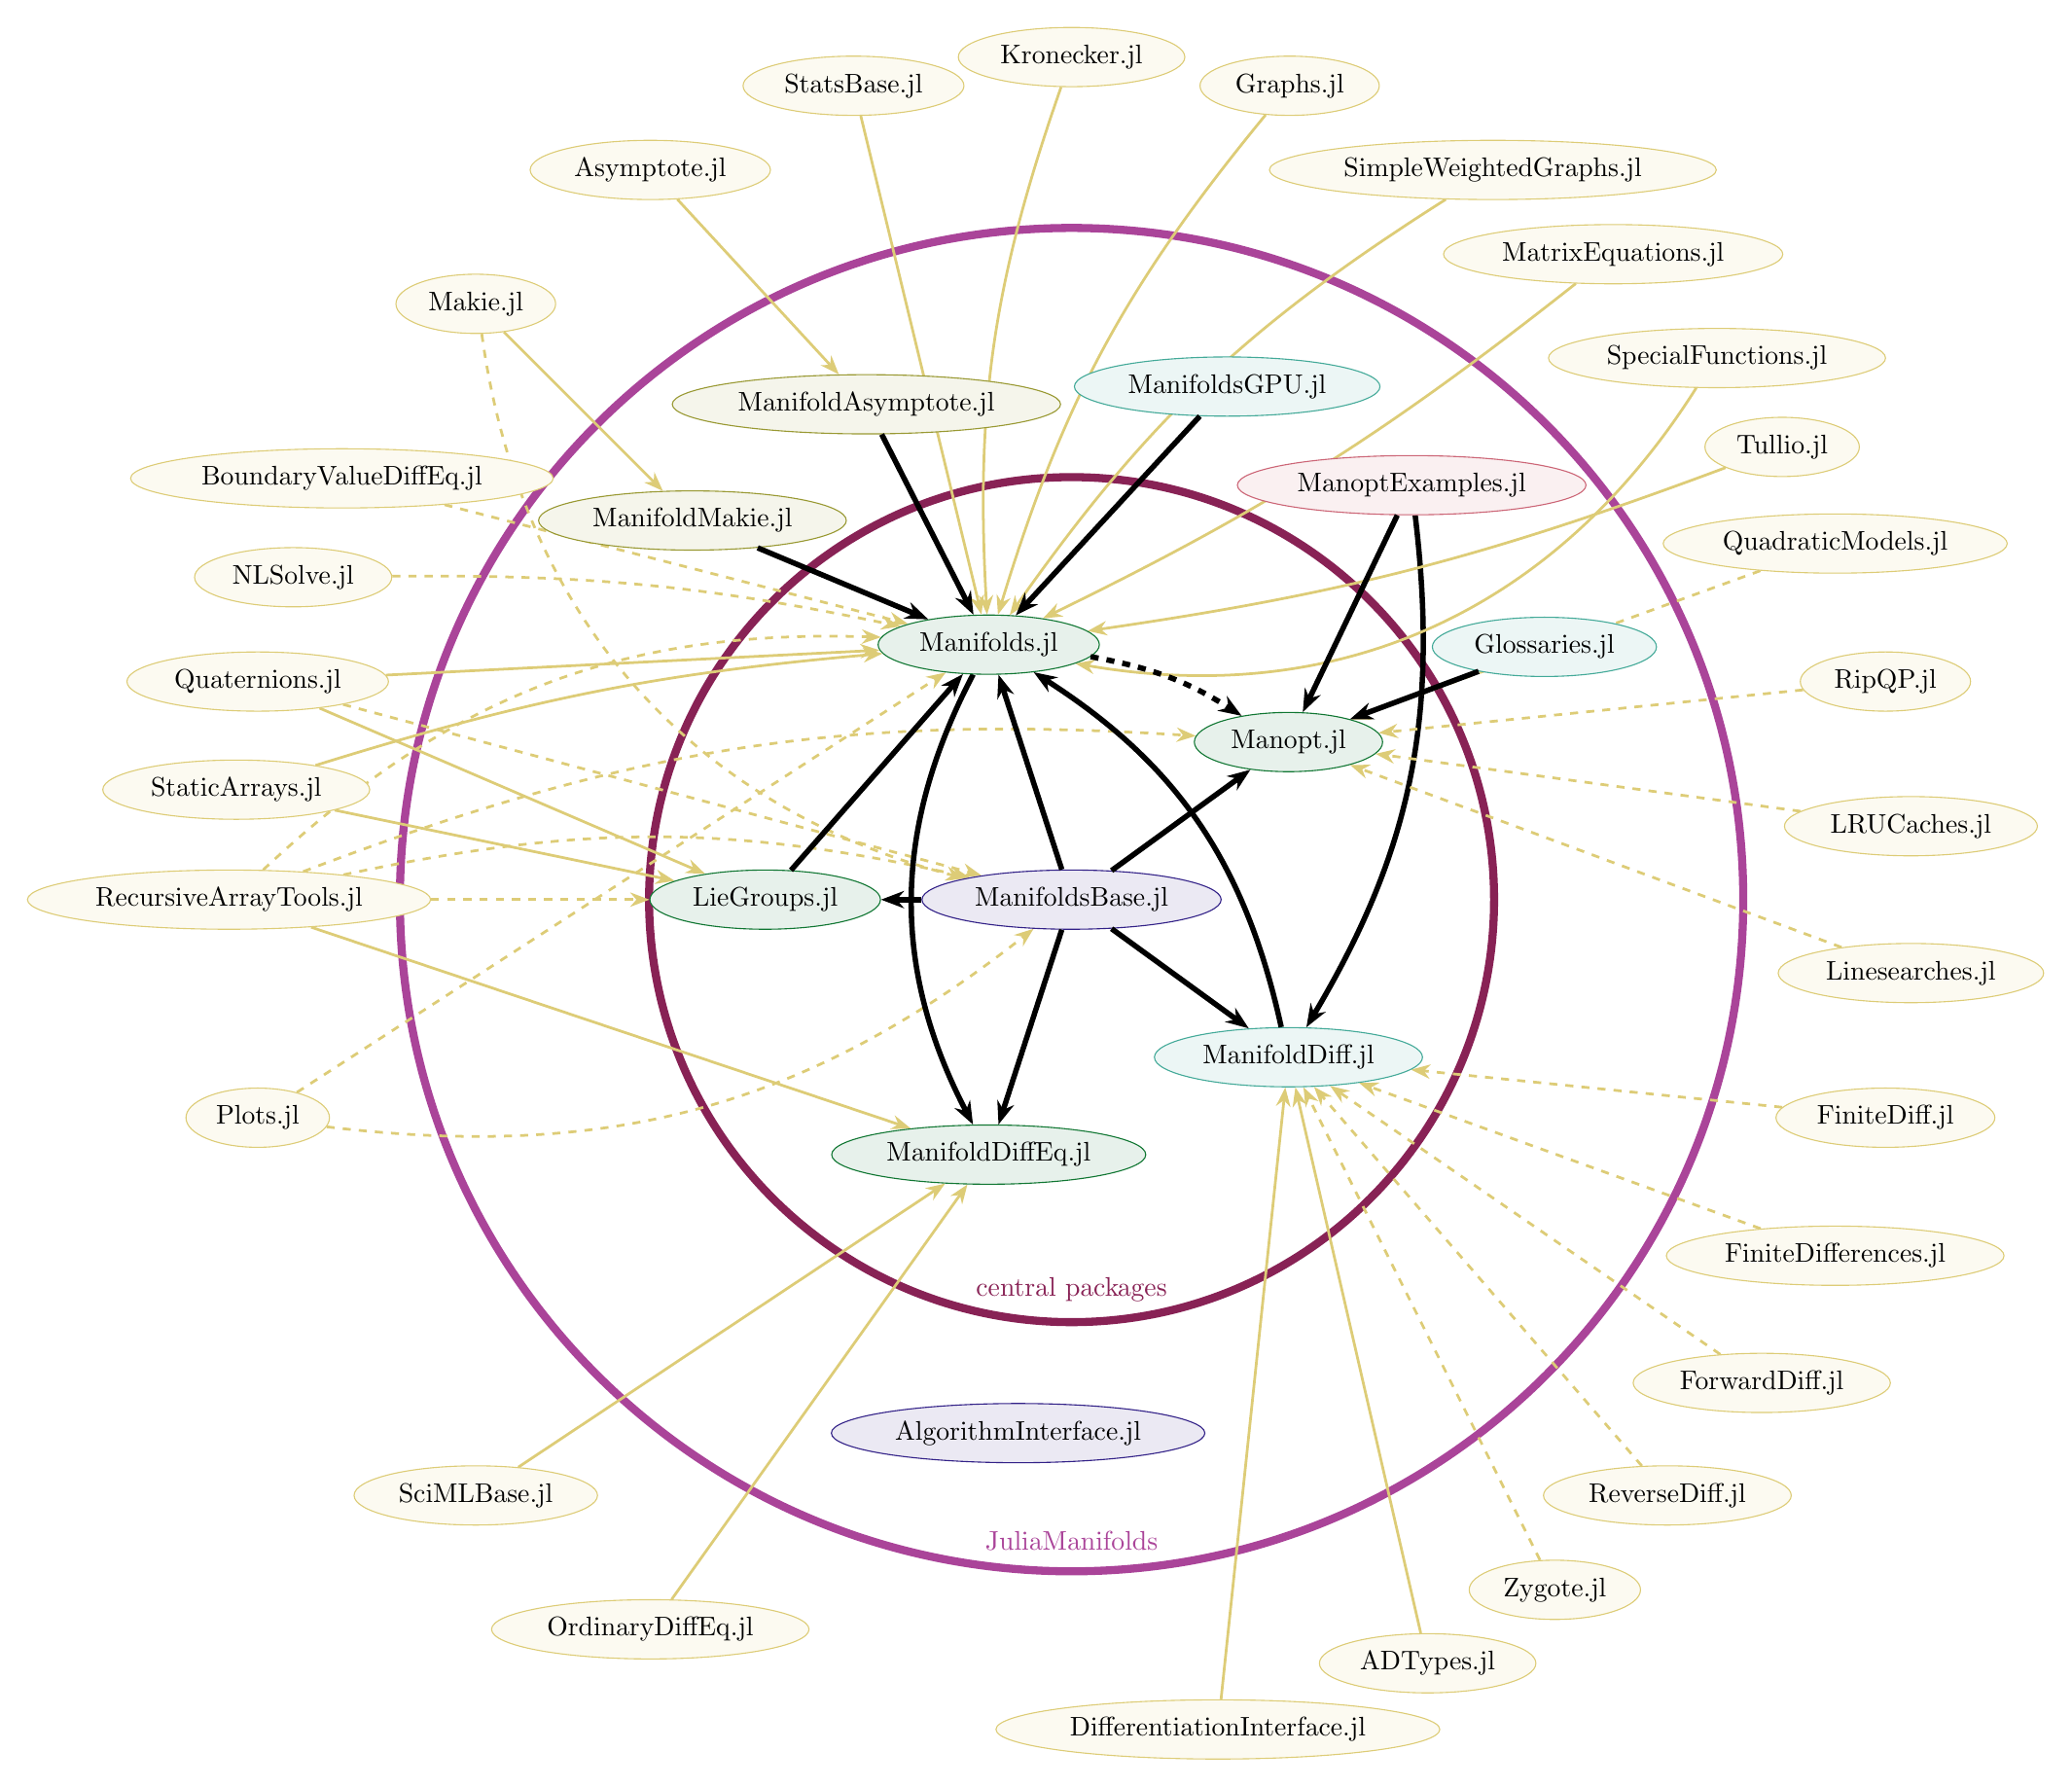
\begin{tikzpicture}[
        %text=white,
        ]
        % Styles of nodes
        \tikzset{Base/.style={draw=TolMutedBlue, fill=TolMutedBlue!10, ellipse}}
        \tikzset{Library/.style={draw=TolMutedGreen, fill=TolMutedGreen!10, ellipse}}
        \tikzset{Func/.style={draw=TolMutedTeal, fill=TolMutedTeal!10, ellipse}}
        \tikzset{Vis/.style={draw=TolMutedOlive, fill=TolMutedOlive!10, ellipse}}
        \tikzset{External/.style={draw=TolMutedSand, fill=TolMutedSand!10, ellipse}}
        \tikzset{Examples/.style={draw=TolMutedRose, fill=TolMutedRose!10, ellipse}}
        % Styles of lines
        % format: a -- B ABExt loading B extends A
        \tikzset{extends/.style={dashed, -{Stealth[length=3mm]}, line width=2pt}}
        % V2: to external packages
        \tikzset{extends2/.style={dashed, -{Stealth[length=2.5mm]},line width=1pt, TolMutedSand}}
        % format A -- B A is a dependency of B, we draw B-->A
        \tikzset{depends/.style={solid, {Stealth[length=3mm]}-,line width=2pt}}
        % V2: to external packages
        \tikzset{depends2/.style={solid, {Stealth[length=2.5mm]}-, line width=1pt, TolMutedSand}}
        \node[Base] (MB) at (0,0) {ManifoldsBase.jl};
        %
        % Ring I: Core packages
        \node[Library] (M) at ($(MB) + (108:3.5cm)$) {Manifolds.jl};
        \node[Library] (MO) at ($(MB) + (36:3.5cm)$) {Manopt.jl};
        \node[Library] (LG) at ($(MB) + (180:4cm)$) {LieGroups.jl};
        \node[Library] (MDE) at ($(MB) + (252:3.5cm)$) {ManifoldDiffEq.jl};
        \node[Func] (MD) at ($(MB) + (324:3.5cm)$) {ManifoldDiff.jl};
        \draw[depends] (M) -- (MB);
        \draw[depends] (MO) -- (MB);
        \draw[depends] (LG) -- (MB);
        \draw[depends] (M) -- (LG);
        \draw[depends] (MDE) -- (MB);
        \draw[depends] (MD) -- (MB);
        \draw[depends] (M) to[bend left=22.5] (MD);
        \draw[extends] (M) to[bend left=11.25] (MO);
        % Ring II
        %
        % Same direction as Manopt continued
        \node[Examples] (MOE) at ($(MB) + (50.625:7cm)$) {ManoptExamples.jl};
        \draw[depends] (MO) -- (MOE);
        %
        % Sidequest: Glossaries
        \node[Func] (G) at ($(MB) + (28.125:7cm)$) {Glossaries.jl};
        \draw[depends] (MO) -- (G);
        \node[Base] (AI) at ($(MB) + (264.275:7cm)$) {AlgorithmInterface.jl};

        %
        % Sidequest Viz
        \node[Vis] (MA) at ($(MB) + (112.5:7cm)$) {ManifoldAsymptote.jl};
        \draw[depends] (M) -- (MA);
        \node[Vis] (MM) at ($(MB) + (135:7cm)$) {ManifoldMakie.jl};
        \draw[depends] (M) -- (MM);
        \node[Func] (MG) at ($(MB) + (73.125:7cm)$) {ManifoldsGPU.jl};
        \draw[depends] (M) -- (MG);
        %
        %
        % Extensions and outer packages on a large circle
        % excluded: Packages from the base language:
        % LinearAlgebra, Markdown, Preferences, Printf, Random, Statistics, Test,
        % Colors, RecipesBase (since we mention PLots)
        % DataStuctures, Dates (Manopt)
        % Consider to add:
        % Accessors, ConstructionBase, DiffEqBase, OrdinaryDiffEqCore, SciMLOperators, SimpleUNpack (ManifoldDiffEq)
        % ScopedValues (for AløgorithmsInterface)
        % Distributions, HybridArrays, DiffEqCallbacks (ext to Manifolds, used in ManoptExamples)
        % Maybe GeometryBasics? dep for ManifoldMakie
        % maybe OffsetArrays (ManoptExtamples)
        \node[External] (LS) at ($(MB) + (355:11)$)  {Linesearches.jl};
        \node[External] (LRU) at ($(MB) + (5:11)$)  {LRUCaches.jl};
        \node[External] (RipQP) at ($(MB) + (15:11)$)  {RipQP.jl};
        \node[External] (QM) at ($(MB) + (25:11)$)  {QuadraticModels.jl};
        \node[External] (Tullio) at ($(MB) + (32.5:11)$)  {Tullio.jl};
        \node[External] (SF) at ($(MB) + (40:11)$)  {SpecialFunctions.jl};
        \node[External] (MatEq) at ($(MB) + (50:11)$)  {MatrixEquations.jl};
        \node[External] (SWG) at ($(MB) + (60:11)$)  {SimpleWeightedGraphs.jl};
        \node[External] (Gr) at ($(MB) + (75:11)$)  {Graphs.jl};
        \node[External] (Kr) at ($(MB) + (90:11)$)  {Kronecker.jl};
        \node[External] (SB) at ($(MB) + (105:11)$)  {StatsBase.jl};
        \node[External] (Asymptote) at ($(MB) + (120:11)$)  {Asymptote.jl};
        \node[External] (Makie) at ($(MB) + (135:11)$)  {Makie.jl};
        \node[External] (MIRK) at ($(MB) + (150:11)$)  {BoundaryValueDiffEq.jl};
        \node[External] (NLS) at ($(MB) + (157.5:11)$)  {NLSolve.jl};
        % \node[External] (Test) at ($(MB) + (165:11)$)  {Test.jl};
        \node[External] (Quat) at ($(MB) + (165:11)$)  {Quaternions.jl};
        \node[External] (SA) at ($(MB) + (172.5:11)$)  {StaticArrays.jl};
        \node[External] (RAT) at ($(MB) + (180:11)$)  {RecursiveArrayTools.jl};
        \node[External] (Plots) at ($(MB) + (195:11)$)  {Plots.jl};
        \node[External] (SLMB) at ($(MB) + (225:11)$)  {SciMLBase.jl};
        \node[External] (ODE) at ($(MB) + (240:11)$)  {OrdinaryDiffEq.jl};
        \node[External] (DI) at ($(MB) + (280:11)$)  {DifferentiationInterface.jl};
        \node[External] (AD) at ($(MB) + (295:11)$)  {ADTypes.jl};
        \node[External] (Z) at ($(MB) + (305:11)$)  {Zygote.jl};
        \node[External] (RD) at ($(MB) + (315:11)$)  {ReverseDiff.jl};
        \node[External] (FD) at ($(MB) + (325:11)$)  {ForwardDiff.jl};
        \node[External] (FiniteDifferences) at ($(MB) + (335:11)$)  {FiniteDifferences.jl};
        \node[External] (FiniteDiff) at ($(MB) + (345:11)$)  {FiniteDiff.jl};
        \draw[depends2] (MA) -- (Asymptote);
        \draw[depends2] (MM) -- (Makie);
        \begin{pgfonlayer}{background}
            \node[circle,
                % fill=TolMutedPurple!10!white,
                draw=TolMutedPurple, line width=3pt,
                inner sep=6.2cm] (JM) at (MB) {};
            \node[circle,
                % fill=TolMutedWine!10!white,
                draw=TolMutedWine, line width=3pt,
                inner sep=3.9cm] (Core) at (MB) {};
            \node[anchor = south, yshift=.2cm, text=TolMutedWine] at (Core.south) {central packages};
            \node[anchor = south, yshift=.2cm, text=TolMutedPurple] at (JM.south) {JuliaManifolds};

            \draw[depends] (MD) to [bend right=18.75] (MOE);
            %
            % \draw[extends2] (Test) -- (M);
            \draw[extends2] (Plots) to[bend right=22.5] (MB);
            \draw[extends2] (Plots) -- (M);
            \draw[extends2] (Makie) to[bend right = 33.75] (MB);
            \draw[extends2] (Quat) -- (MB);
            \draw[extends2] (RAT) to[bend left=22.5] (M);
            \draw[extends2] (NLS) to[bend left=6.125] (M);
            \draw[extends2] (MIRK) -- (M);
            \draw[extends2] (RAT) to[bend left=12.25] (MB);
            %
            \draw[depends2] (M) to[bend right = 0] (Quat);
            \draw[depends2] (M) to[bend left = 11.25] (Gr);
            \draw[depends2] (M) to[bend left = 11.25] (Kr);
            \draw[depends2] (M) to[bend left = 11.25] (SWG);
            \draw[depends2] (M) to[bend right = 33.75] (SF);
            \draw[depends2] (M) to[bend right = 6.125] (Tullio);
            \draw[depends2] (M) to[bend left = 0] (SB);
            \draw[depends2] (M) to [bend right = 6.125] (MatEq);
            \draw[depends2] (M) to [bend right = 6.125] (SA);
            \draw[depends2] (LG) to [bend left = 0] (SA);
            \draw[depends2] (LG) -- (Quat);
            % Manopt extensions
            \draw[extends2] (RAT) to[bend left=12.25] (MO);
            \draw[extends2] (RipQP) -- (MO);
            \draw[extends2] (QM) -- (MO);
            \draw[extends2] (LRU) -- (MO);
            \draw[extends2] (LS) -- (MO);
            % LieGroups extensions
            \draw[extends2] (RAT) -- (LG);
            % \draw[extends2] (Test) -- (LG);
            % ManifoldDiff dependencies
            \draw[depends2] (MD) -- (AD);
            \draw[depends2] (MD) -- (DI);
            % ManifoldDiff weakdependencies
            \draw[extends2] (FiniteDiff) -- (MD);
            \draw[extends2] (FiniteDifferences) -- (MD);
            \draw[extends2] (FD) -- (MD);
            \draw[extends2] (RD) -- (MD);
            \draw[extends2] (Z) -- (MD);
            % ManifoldDiffEq dependencies
            \draw[depends] (MDE) to[bend left=27.625] (M);
            \draw[depends2] (MDE) -- (ODE);
            \draw[depends2] (MDE) to [bend left=0] (RAT);
            \draw[depends2] (MDE) -- (SLMB);
        \end{pgfonlayer}
    \end{tikzpicture}
\end{document}